\section{Alignment Function}
\begin{frame}[allowframebreaks]{Alignment Function}
    \begin{itemize}
        \setlength{\itemsep}{0.5em}
        \item The alignment function is a crucial component of attention mechanisms, determining how much focus to place on different parts of the input sequence.
        \item It computes a score for each input token relative to the current output token being generated.
        \item The scores are then normalized (often using softmax) to create a probability distribution, indicating the relative importance of each input token.
        \item Common alignment functions include:
        \begin{itemize}
            \item \textbf{Dot Product}: Computes the dot product between the query and key vectors.
            \item \textbf{Scaled Dot Product}: Similar to dot product but scaled by the square root of the dimension of the key vectors to prevent large values that can saturate the softmax function.
            \item \textbf{Additive Attention}: Combines the query and key vectors using a feed-forward neural network to compute the alignment scores.
        \end{itemize}
    
        \item The choice of alignment function can significantly impact the model's performance, especially in tasks with long sequences or complex dependencies.
    \end{itemize}
    \textbf{Example:} In a translation task, the alignment function helps the model determine which words in the source language should be emphasized when generating each word in the target language. For instance, when translating "The cat sat on the mat," the model might focus more on "cat" when generating "gato" in Spanish, while still considering "sat" and "on" to maintain the context.
\end{frame}

\begin{frame}{Types of Alignment Functions}
    \begin{itemize}
        \item \textbf{Dot Product:}
        \[
            \text{score} = q^\top k
        \]
        \item \textbf{Scaled Dot Product:}
        \[
            \text{score} = \frac{q^\top k}{\sqrt{d_k}}
        \]
        (used in Transformers to prevent softmax saturation)
        \item \textbf{Additive (Bahdanau) Attention:}
        \[
            \text{score} = v^\top \tanh(W_1 h_i + W_2 s_t)
        \]
        \item \textbf{General:}
        \[
            \text{score} = q^\top W k
        \]
    \end{itemize}
    \vspace{0.5em}
    \textbf{\faThumbTack\hspace{0.5em}Each function balances efficiency vs expressiveness.}
\end{frame}

\begin{frame}{Attention Model}
    \begin{figure}
        \centering
        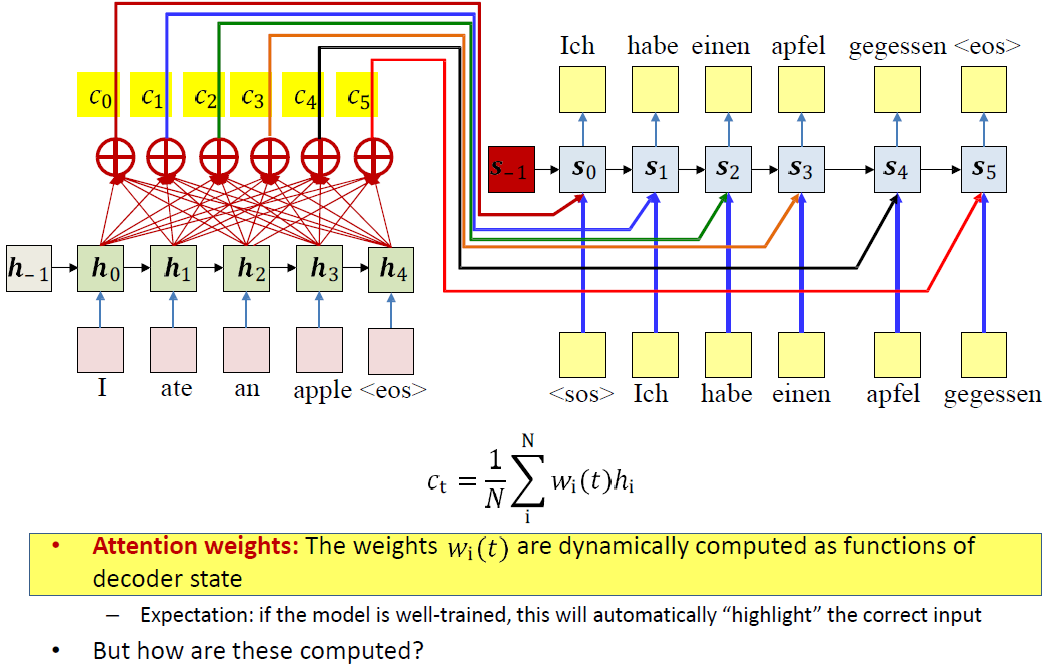
\includegraphics[width=\textwidth]{images/attention/attention-1.png}
    \end{figure}
\end{frame}

\begin{frame}{Attention weights at time}
    \begin{figure}
        \centering
        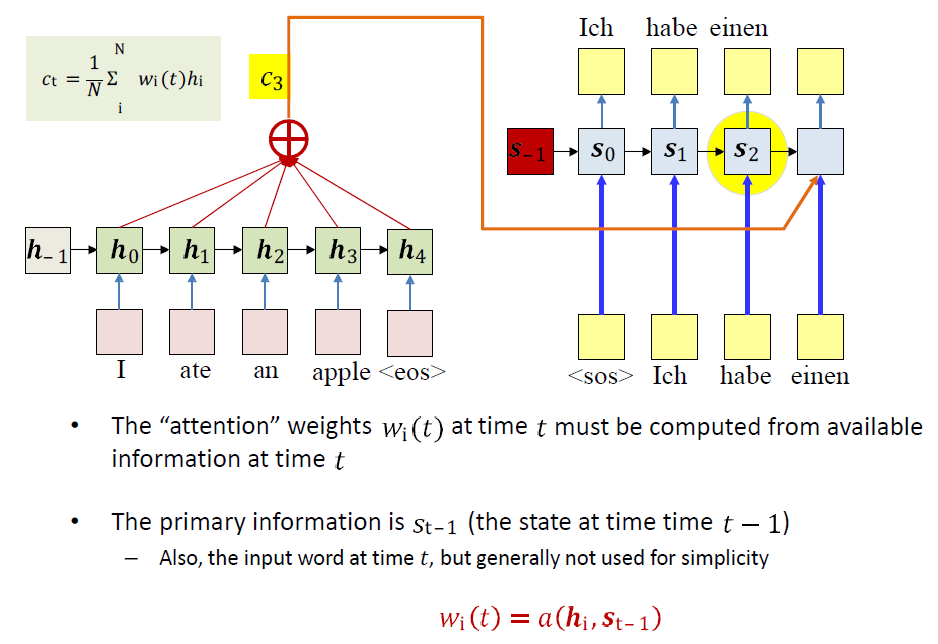
\includegraphics[width=\textwidth]{images/attention/attention-2.png}
    \end{figure}
\end{frame}

\begin{frame}[allowframebreaks]{Requirement on attention weights}
    \begin{figure}
        \centering
        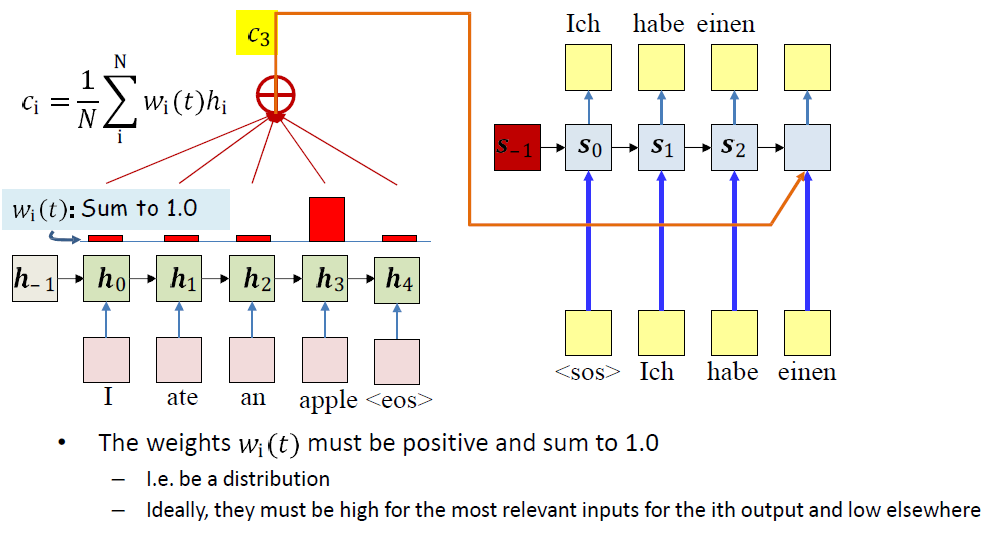
\includegraphics[width=\textwidth]{images/attention/attention-3.png}
    \end{figure}
\framebreak
    \begin{figure}
        \centering
        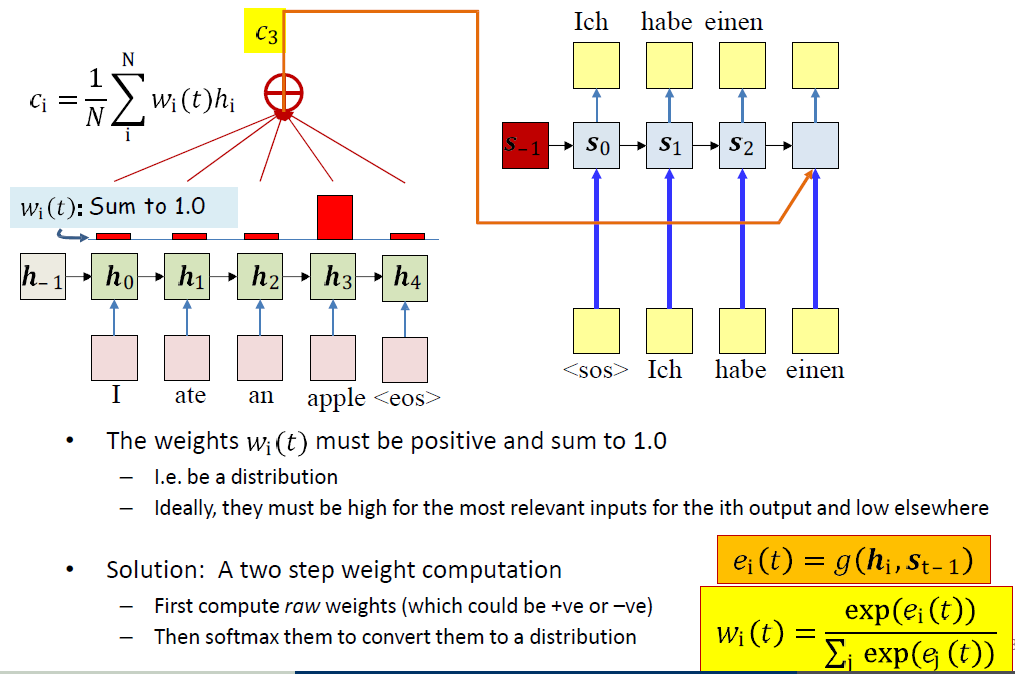
\includegraphics[width=\textwidth]{images/attention/attention-4.png}
    \end{figure}
\framebreak
    \begin{figure}
        \centering
        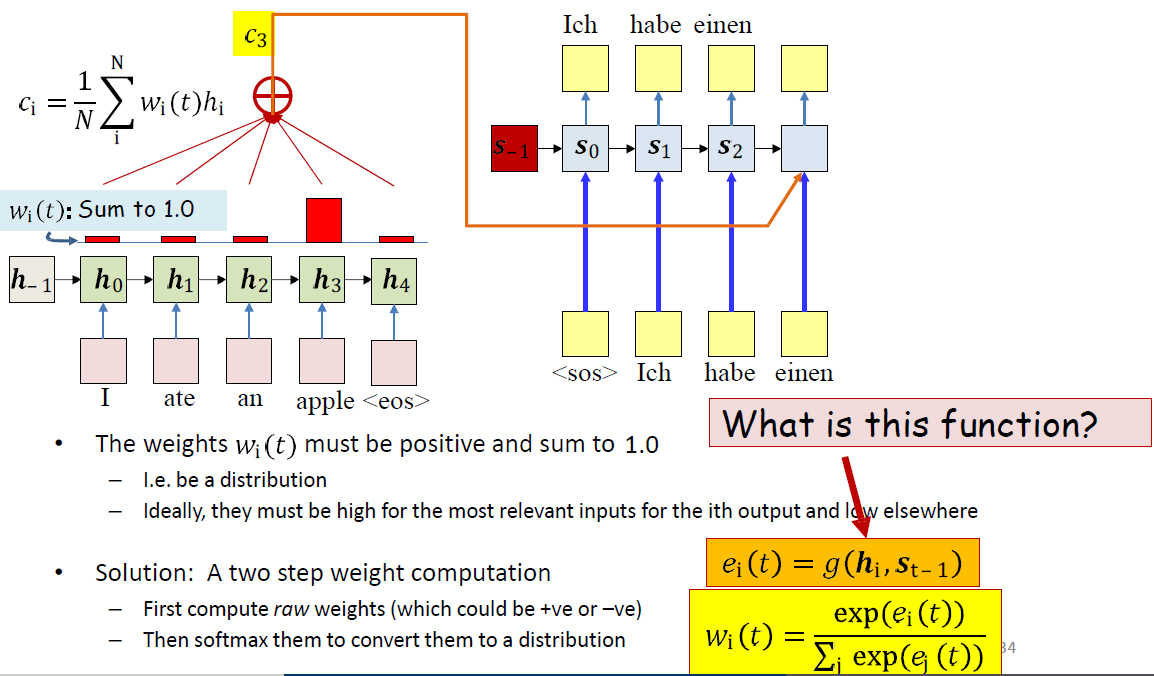
\includegraphics[width=\textwidth]{images/attention/attention-5.png}
    \end{figure}
\end{frame}

\begin{frame}[allowframebreaks]{Attention weights}
    \begin{figure}
        \centering
        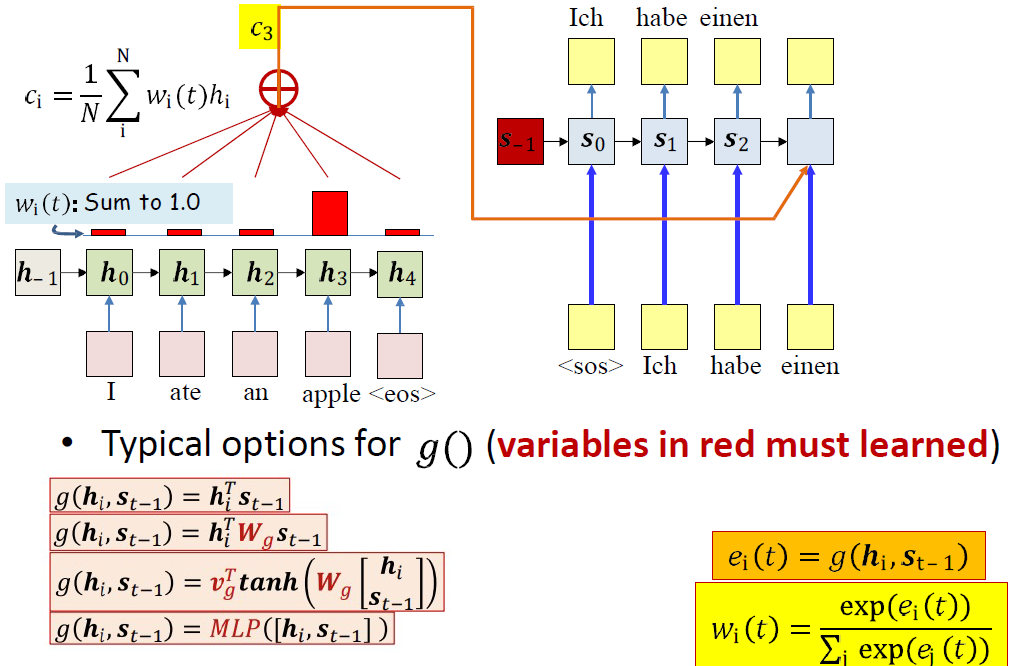
\includegraphics[width=\textwidth]{images/attention/attention-6.png}
    \end{figure}
\framebreak
    \begin{figure}
        \centering
        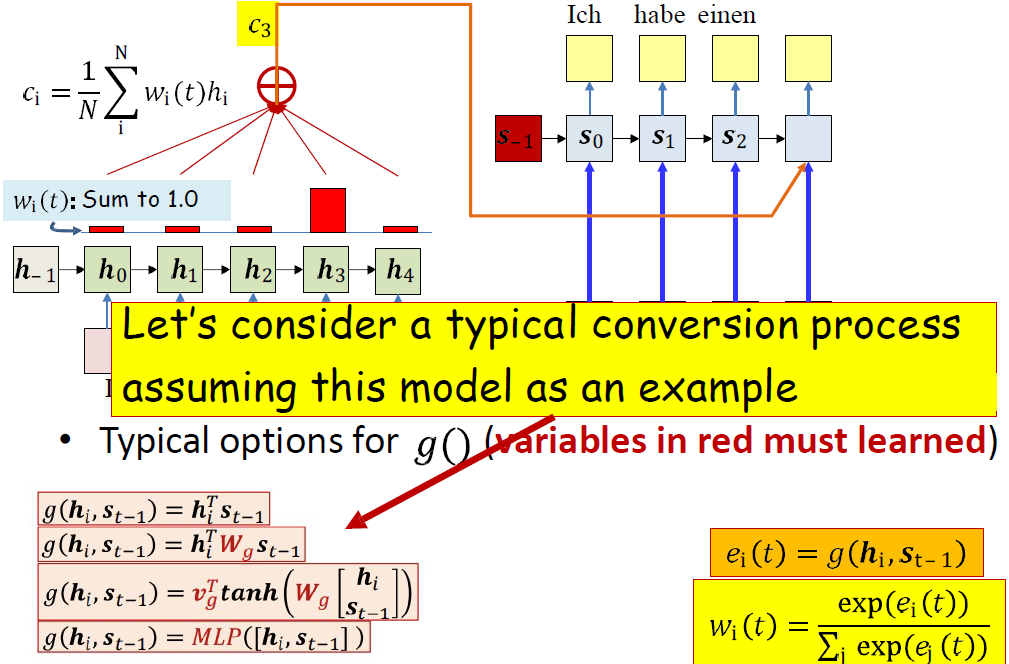
\includegraphics[width=\textwidth]{images/attention/attention-7.png}
    \end{figure}
\end{frame}
